\documentclass[10pt]{article}
\usepackage{icmlko}

\icmlmeta{IP 파운데이션 월드모델}{173}{한쪽만 채우면 무너진다}{과제 82 --- 학습 구간까지 읽어 채우면 전이 손실이 회수되나. 19\%가 회수되고 그것도 안 갈리는데, 대신 한쪽만 채우면 어떻게 되는지는 아주 분명하게 갈린다}

\begin{document}

\twocolumn[
\icmlheader

\begin{abstract}
노트 154가 시장 레코드를 읽어 매긴 축이 \emph{따로} 재면 $\rho{=}+0.374$
인데 하네스 안에서는 $+0.197$ 만 나온다는 것을 보이고, 그 차이를 전이
손실(47\%)로 불렀다 --- 풀링 모형이 내부 레코드(676자 기획서)로만 적합돼
시장 레코드(158자 기사)의 눈금을 모른다는 읽기였다. 과제 82가 그 처방이다:
\textbf{학습 구간의 시장 레코드도 읽어 채운다.} 57건을 눈가림으로 매겨
(유보분 51건과 합쳐 108건) 넣고 쟀다. \textbf{회수된다 --- 다만 조금이고
안 갈린다.} 늘어난 51건의 $\rho$ 가 $+0.197$ 에서 \textbf{$+0.231$} 로,
팝업 전체가 $+0.275$ 에서 \textbf{$+0.309$} 로 오른다. 간격 0.177의
\textbf{19\%} 이고 $+0.034 \pm 0.044$($t{=}0.8$)로 안 갈린다.
\textbf{판 $\rho$ 는 $+0.4385$에서 $+0.4486$ 으로 올라 표준 59 기준선
($+0.4462$)을 넘는다} --- 유보 표본이 두 배인 채로 판이 안 나빠진다는
뜻이라 노트 154가 세운 ``두 분모를 나란히 적는다''의 근거가 하나 는다.
\textbf{그런데 이 실험의 제일 뚜렷한 값은 대조군에서 나왔다.} 학습 구간만
채우고 유보는 비워 두면 팝업 $\rho$ 가 \textbf{$-0.018$} 이다 --- $+0.275$
에서 0.29 떨어진다. 모형이 손 축에 기대는 법을 배운 뒤 예측 시점에 그
축이 없으면 무너진다. \textbf{채움은 시간 분할의 양쪽에 대칭이어야 한다}
--- 한쪽만 채우는 것은 안 채우는 것보다 훨씬 나쁘다.
\end{abstract}
]

\begin{figure*}[t]
\centering
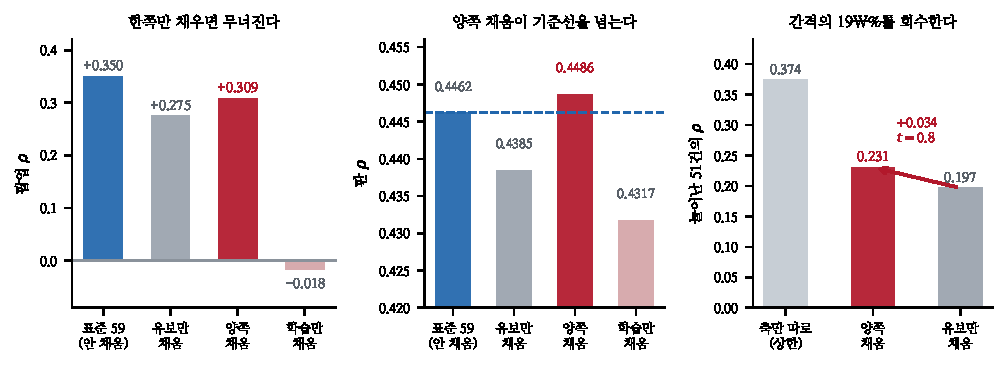
\includegraphics[width=\textwidth]{figs/both.pdf}
\caption{왼쪽 --- 한쪽만 채우면 무너진다. 가운데 --- 양쪽 채움이 기준선을
넘는다. 오른쪽 --- 간격의 19\%를 회수한다.}
\end{figure*}

\section{네 판}

\begin{table}[t]
\centering\tsize
\caption{F18 배깅 · 씨앗 셋 평균. 채운 행은 내가 읽어 매긴 것.}
\begin{tabular}{lrrrr}
\toprule
& 채운 행 & 유보 n & 팝업 $\rho$ & 판 $\rho$ \\
\midrule
표준 59 & 0 & 59 & $+$.3505 & $+$.4462 \\
유보만 채움 & 51 & 116 & $+$.2751 & $+$.4385 \\
\textbf{양쪽 채움} & \textbf{108} & 116 & \textbf{$+$.3086} & \textbf{$+$.4486} \\
\textbf{학습만 채움} & 57 & 116 & \textbf{$-$.0180} & $+$.4317 \\
\bottomrule
\end{tabular}
\end{table}

\section{회수는 19퍼센트}

\begin{table}[t]
\centering\tsize
\caption{늘어난 51건에서만.}
\begin{tabular}{lrl}
\toprule
축만 따로 (노트 154) & $+$.374 & 상한 \\
\midrule
유보만 채움 & $+$.197 & \\
\textbf{양쪽 채움} & \textbf{$+$.231} & $+$.034 \\
\bottomrule
\end{tabular}
\end{table}

\claimx{\textbf{간격의 19\%가 회수된다.} 0.374와 0.197의 차 0.177 중
0.034다. 방향은 처방대로다 --- 학습 쪽에도 시장 레코드의 눈금을 보여
주면 전이가 조금 나아진다.}{$+0.034 \pm 0.044$($t{=}0.8$)로 안 갈린다.
51건에서 이만한 차이를 가르려면 표본이 네 배쯤 필요하다.}

\claimx{\textbf{남은 81\%는 학습 표본으로는 안 메워질 수 있다.} 내부
기획서는 676자이고 시장 기사는 158자다 --- 눈금 문제가 아니라 정보량
문제라면 학습을 아무리 늘려도 안 메워진다.}{가르려면 같은 팝업의 기획서와
기사를 둘 다 가진 건이 필요한데, 시장 레코드는 정의상 내부 건이 아니다.
\textbf{이 판에서는 못 가른다.}}

\section{판은 기준선을 넘는다}

\claimx{\textbf{양쪽 채움의 판 $\rho$ 가 $+$0.4486으로 표준 59
기준선($+$0.4462)을 넘는다.} 유보 표본을 59에서 116으로 두 배 늘리면서
판이 안 나빠진다.}{$+$0.0024 차이라 갈리지는 않는다. 요점은 ``더 낫다''가
아니라 \textbf{``더 큰 표본을 공짜로 얻는다''} 이다 --- 노트 154가 잰
대로 116 분모는 짝 sd 가 20$\sim$40\% 좁다.}

\section{대조군이 제일 뚜렷하다}

\claimx{\textbf{학습만 채우면 팝업 $\rho$ 가 $-$0.018이다} --- $+$0.275
에서 0.29 떨어진다. 어떤 오차막대로도 안 덮인다.}{모형이 학습에서 손 축에
기대는 법을 배우는데 유보 51건에는 그 축이 없다(마스크 0). \textbf{예측
시점에 없는 것에 기대게 만든 것이다.}}

\claimx{\textbf{규약: 채움은 시간 분할의 양쪽에 대칭이어야 한다.} 한쪽만
채우는 것은 안 채우는 것보다 훨씬 나쁘다 --- $+$0.275 대 $-$0.018이다.}{노트
133이 학습 풀을 넓힐 때 축을 안 채운 것은 결과적으로 옳았다. 그때 채웠으면
반대쪽 비대칭이 됐을 것이다.}

\begin{table}[t]
\centering\tsize
\caption{남은 것.}
\begin{tabular}{ll}
\toprule
81\% & 정보량 문제인지 눈금 문제인지 못 가른다 \\
분모 & 116 을 정식 분모로 올릴 것인가 \\
\textbf{다음} & 팝업 밖 --- 나머지 아홉 도메인의 빈칸 \\
\bottomrule
\end{tabular}
\end{table}

마지막 줄이 다음이다. 이 노트는 팝업의 빈칸만 봤다. 노트 168이 적은 대로
다른 도메인에도 마스크 0인 축이 많다 --- 특히 미디어 푸시는 다섯 도메인이
통째로 비어 있다(노트 163에서 칸이 넷뿐이었던 이유다). \textbf{같은 방식으로
채울 수 있는지가 다음 자리다.}

\end{document}
